\section{Implementación del prototipo}\label{section:prototype}

El prototipo implementado se concibe como una aplicaci\'on web. Se compone de cuatro componentes: Crawler, Cat\'alogo de Datos, Generador de Consultas 
e Interfaz de Usuario; los cuales se corresponden al diseño de sistema propuesto en el cap\'itulo \ref{chapter:proposal}. 
La l\'ogica de los an\'alisis sintáctico y l\'exico del DSL propuesto fue incluida dentro del Generador de Consultas. 
Por cuestiones de tiempo no se pudo concretar una implementaci\'on del Generador de Pipelines.

\subsection{Organización de los archivos}

La l\'ogica de cada uno de los componentes de la aplicaci\'on se encuentra separada por carpetas. Cada componente 
posee su propia carpeta identificada con el nombre del componente en ingl\'es, a excepción de la Interfaz de Usuario 
cuya carpeta es nombrada \textbf{pages} y su script principal se encuentra en la ra\'iz del proyecto con el nombre de 
\textbf{MainPage.py}. Todos los datos derivados de la ejecución de la l\'ogica de cada uno de los componentes 
se almacena dentro de la carpeta \textbf{data}. La carpeta \textbf{utils} guarda scripts de algoritmos usados 
en varias partes de la aplicaci\'on, concretamente posee scripts con algoritmos para la carga y escritura de los 
grafos y \'arboles de join en el disco.

\subsection{Fuentes de datos}

El prototipo solo es capaz de manejar una sola fuente de datos a la vez, aunque si se pueden considerar varias 
fuentes de datos para un mismo almac\'en de datos de destino. Para esto se debe definir un script del DSL por 
cada fuente de datos que alimente el almac\'en de datos. Las primeras consultas de creación generadas que se ejecuten 
para dicho almac\'en de datos van a determinar el nombre de las dimensiones y tablas de hechos, as\'i como 
como el nombre de sus atributos, sus tipos y restricciones. Luego, para alimentar el almac\'en de datos con otras 
fuentes basta con ejecutar solamente las consultas de selecci\'on generadas a partir del script correspondiente a 
dicha fuente y luego insertar en el almac\'en los valores extra\'idos.

\subsection{Crawler}

El Crawler constituye un elemento de interdependencia dentro del prototipo en relación con los sistemas 
de gestión de bases de datos, específicamente con los SGBD de las fuentes de datos. Con el objetivo de lograr una 
mayor extensibilidad, se plantea la creación de una clase abstracta llamada \textbf{crawler}, la cual establecerá 
el comportamiento general de este componente. De este modo, se delega a las implementaciones específicas para cada 
SGBD la definición de la forma en que se llevan a cabo las operaciones, como se muestra en la figura \ref{fig:crawler}.
A continuación de se muestra la definición de la clase crawler.

\begin{lstlisting}[label={code:crawler}, caption={clase abstracta crawler}, language={python}]
    import abc

    class Crawler(metaclass=abc.ABCMeta):
        def __init__(self, dbname, user, password, host, port) -> None:
            self.dbname = dbname
            self.user = user
            self.password = password
            self.host = host
            self.port = port
            self._db_params = {'dbname': dbname, 'user': user, 'password': password, 'host': host, 'port': port}
            self._metadata_str = ''
            self._db_dict = {}

        @abc.abstractmethod
        def explore_db(self):
            pass
        
        @abc.abstractmethod
        def export_metadata_to_file(self):
            pass

\end{lstlisting}

La definición de esta clase se encuentra en el archivo \textbf{crawler.py} de la carpeta del componente. Los 
campos de la clase se corresponden con la informaci\'on necesaria para establecer una conexi\'on con una base de 
datos. 

El m\'etodo \textbf{explore\_db} se encarga de recopilar los metadatos mencionados en el cap\'itulo \ref{chapter:proposal}
y almacenarlos en el diccionario \textbf{\_db\_dict} el cual tiene como llaves los nombres de las tablas de la base 
de datos y como valores otros diccionarios que poseen dos llaves: \textbf{attributes} y \textbf{relations}. 
El valor de \textbf{attributes} es una lista de tuplas de dos o tres elementos, una por cada atributo de la tabla. 
Las tuplas de dos elementos almacenan el nombre del atributo y el tipo, las de tres almacenan adem\'as un indicador 
que expresa si el atributo es llave primaria, for\'anea o ambas. El valor de \textbf{relations} es una lista de 
tuplas de tres elementos, una por cada atributo llave for\'anea de la tabla. El primer elemento es el nombre 
de la llave for\'anea en la tabla, el segundo el nombre de la tabla referenciada y el tercero el atributo referenciado. 
Adem\'as, el m\'etodo \textbf{explore\_db} tiene la responsabilidad de llenar la cadena de texto \textbf{\_metadata\_str} 
que almacena los metadatos recopilados en un formato m\'as expresivo para luego ser mostrado al usuario.

El m\'etodo \textbf{export\_metadata\_to\_file} se encarga guardar \textbf{\_db\_dict} y \textbf{\_metadata\_str} en el disco, 
en la ruta \textbf{data/schemas}. La carpeta \textbf{schemas} contiene una carpeta por cada base de datos identificada 
por el nombre de dicha base de datos en la cual se almacena en formato json \textbf{\_db\_dict} y en formato txt 
\textbf{\_metadata\_str}.

En esta primera entrega del prototipo solo se le di\'o implementaci\'on a un crawler para PostgreSQL. Su l\'ogica 
se encuentra en el archivo \textbf{postgreSQL\_crawler.py}. Los metadatos son recopilados mediante consultas realizadas
a la tabla \textbf{information\_schema} de base de datos fuente ejecutadas 
utilizando el adaptador de PostgreSQL para python \textbf{psycopg2}.

\begin{figure}[htb]
    \centering
    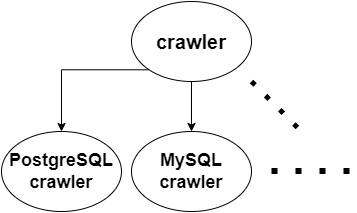
\includegraphics[width=0.5\textwidth]{Graphics/crawler_class.drawio.png}
    \caption{Jerarqu\'ia de la clase abstracta crawler}
    \label{fig:crawler}
\end{figure}


\subsection{Cat\'alogo de Datos}

El Cat\'alogo de Datos es un servido de base de datos de Neo4j. La idea es que exista un base de datos Neo4j por cada 
fuente de datos, sin embargo la versi\'on community de Neo4j utilizada solo permite la creación de una sola base de datos. 
Por tanto, cada vez que se establece conexi\'on con otra base de datos fuente la informaci\'on existente en cat\'alogo es 
sobreescrita. Esto no supone un problema para la inferencia de Joins puesto que el grafo de join obtenido a partir 
del Cat\'alogo de Datos es almacenado en el disco y recuperado cuando es necesario su uso. Para versiones m\'as avanzadas 
del prototipo se debe considerar la utilizaci\'on de Neo4j Enterprise.

La comunicaci\'on de la aplicaci\'on con el Cat\'alogo de Datos es mediada por la clase \textbf{DataCatalogHandler} 
presente en el script \textbf{handler.py} de la carpeta \textbf{data\_catalog}. A continuación se muestra parte 
del c\'odigo de dicha clase.

\begin{lstlisting}[label={code:catalog}, caption={Clase DataCatalogHandler}, language={python}]
    class DataCatalogHandler():
        def __init__(self, db_dict, db_name, user, password, uri) -> None:
            self.db_dict = db_dict
            self._user = user
            self._password = password
            self._uri = uri
            self.db_name = db_name
            self.join_graph = None

        def create_graph_database(self):
            # Omitted implementation

        def export_join_graph(self):
            # Omitted implementation

\end{lstlisting}

El campo \textbf{db\_dict} es el diccionario de la base de datos confeccionado por el Crawler, \textbf{db\_name} es 
nombre de la base de datos fuente, \textbf{join\_graph} almacena el grafo de join derivado y el resto de atributos 
son los necesarios para establecer una conexi\'on con una base de datos de Neo4j, en especial, el campo \textbf{\_uri} 
es una cadena de texto que contiene el protocolo de comunicaci\'on con el servidor de Neo4j, su ip y su puerto. 

El m\'etodo \textbf{create\_graph\_database} crea en la base de datos de Neo4j dedicada a la fuente de datos con nombre 
\textbf{db\_name} y con diccionario de metadatos \textbf{db\_dict} un nodo por cada llave (tabla) 
en \textbf{db\_dict} con las propiedades \textbf{name} que almacena el nombre de la tabla, \textbf{pks} que es una 
lista con los nombres de los atributos que son llaves primarias y por \'ultimo \textbf{attributes} que 
es la lista tuplas correspondiente a la llave attributes del diccionario que contiene \textbf{db\_dict} 
indexado en el nombre de la tabla en cuesti\'on. Adem\'as, se crea una relación direccionada por cada por cada llave for\'anea 
presente en la lista correspondiente a la llave relations del diccionario que contiene \textbf{db\_dict} 
indexado en el nombre de la tabla en cuesti\'on. La direcci\'on de la relación la dictamina la direcci\'on de la llave 
for\'anea, tal y como se expuso en el capitulo \ref{chapter:proposal}

El m\'etodo \textbf{export\_join\_graph} es el encargado de construir, a partir de la base de datos Neo4j del esquema 
de la fuente de turno, el grafo de join. Mediante el lenguaje de consulta Cypher y el adaptador de Neo4j para python 
se extraen todos los nodos y relaciones y se crea un digrafo de NetworkX equivalente, que adem\'as conserva las 
propiedades definidas para nodos y relaciones, este digrafo es el grafo de join. Se le añaden adem\'as arcos 
adicionales siguiendo la teor\'ia expuesta para el grafo de join en el capitulo \ref{chapter:proposal}. Luego 
de creado el grafo de join se almacena en la ruta \textbf{data/join\_graphs} con el nombre de la base de datos fuente 
que representa.


\subsection{Generador de Consultas}

El generador de consultas est\'a compuesto por la l\'ogica para el tratamiento de los scripts del lenguaje de 
dominio espec\'ifico y generaci\'on de consultas, y por la l\'ogica del computo relacionado a los \'arboles de join. 
Esta \'ultima se encuentra en los scripts \textbf{maximal\_join\_trees.py}, \textbf{join\_computation.py} y 
\textbf{all\_spanning\_trees.py}. En el primero yace, con el nombre de \textbf{maximal\_join\_trees\_generator}, 
la implementaci\'on en python del pseudoc\'odigo propuesto para la generaci\'on de los \'arboles de join en el 
cap\'itulo \ref{chapter:proposal}. Luego de generados los \'arboeles de join son almacenados en la ruta 
\textbf{data/join\_trees}

Por simplicidad, se utiliza para la obtenci\'on de los \'arboles en expansi\'on de los grafos alcanzables el algoritmo 
provisto por NetworkX para este fin. Los \'arboles de join son digrafos de NetworkX. Adem\'as, se les añade las propiedades 
\textbf{root} que identifica a la ra\'iz del \'arbol y a cada nodo se le añade la propiedad \textbf{height} que almacena 
la altura del nodo con respecto a la ra\'iz del \'arbol.

En script \textbf{all\_spanning\_trees.py} yacen los algoritmo para la obtenci\'on de los \'arboles de expansi\'on 
de un grafo alcanzable. En esta primera entrega solo se le di\'o implementaci\'on a una variante que se apoya de la 
clase ArborescenceIterator de NetworkX la cual constituye un iterador de los \'arboles de expansi\'on de un digrafo 
pasado como argumento.

El script \textbf{join\_computation.py} alberga el algoritmo \textbf{compute\_joins} el cual es la implementaci\'on 
en python del algoritmo \textbf{get\_joins} cuyo pseudoc\'odigo fue expuesto en el cap\'itulo \ref{chapter:proposal}. 
Este algoritmo recibe la lista de \'arboeles de joins y una lista de tablas a unir y devuelve una lista de joins.

\subsubsection{Lenguaje de Dominio Espec\'ifico}

La l\'ogica del DSL se encuentra en la ruta \textbf{query\_generator/dsl}. La biblioteca 
PLY demanda la creaci\'on de dos scripts, uno donde se especifiquen los terminales de la gram\'atica y las reglas 
para el an\'alisis l\'exico, y otro donde se especifiquen las producciones de la gram\'atica mediante funciones. Estos 
scripts son \textbf{lexer.py} y \textbf{parser\_rules.py} respectivamente. En el script \textbf{ast\_nodes.py} se define  
la jerarqu\'ia de clases de los nodos del \'arbol de sintaxis abstracta (AST) del lenguaje de dominio espec\'ifico. Cada 
estructura gramatical del lenguaje est\'a representada por una clase, como se muestra en la figura \ref{fig:ast}.

\begin{figure}[htb]
    \centering
    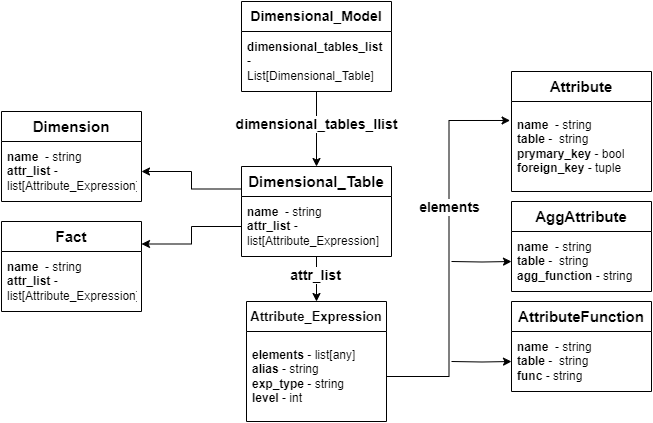
\includegraphics[width=0.7\textwidth]{Graphics/ast.png}
    \caption{Estructura del AST}
    \label{fig:ast}
\end{figure}

La clase \textbf{Dimensional\_Model} representa un modelo dimensional el cual est\'a formado por una lista de tablas 
dimensionales \textbf{Dimensional\_Table}. Las clases \textbf{Dimension} y \textbf{Fact} heredan de \textbf{Dimensional\_Table} 
y representan a las dimensiones y a las tablas de hecho respectivamente. La clase \textbf{Attribute\_Expression} expresa 
la definici\'on de un atributo, ya sea simple o una expresi\'on aritm\'etica donde participen varios atributos y n\'umeros. 
Las clases \textbf{Attribute}, \textbf{AggAttribute} y \textbf{AttributeFunction} representan atributos simples, atributos 
agregados y atributos resultado de la aplicación de alguna funci\'on respectivamente. El campo \textbf{foreign\_key} de 
la clas \textbf{Attribute}, en caso de tener alg\'un valor almacenado, es una tupla que indica que la la instancia 
de \textbf{Attribute} es una llave for\'anea y en la primera posici\'on almacena el nombre de la tabla referenciada y 
en la segunda posici\'on el nombre del atributo referenciado.

Una instancia de \textbf{Dimensional\_Model} contiene una lista de instancias de \textbf{Dimensional\_Table}, que a su vez pueden ser de tipo 
\textbf{Dimension} o \textbf{Fact}. Adem\'as, posee una lista de instancias de \textbf{Attribute\_Expression}, cada 
una de ellas presenta 
una lista llamada \textbf{elements} que puede contener uno o varios elementos, en caso de tener solo un elemento 
este es una instancia de \textbf{Attribute}, \textbf{AggAttribute} o \textbf{AttributeFunction}; en caso de tener 
m\'as de un elemento, es decir, la instancia de \textbf{Attribute\_Expression} representa un atributo compuesto entonces 
elements contiene tanto las instancias de \textbf{Attribute}, \textbf{AggAttribute} o \textbf{AttributeFunction} como 
los signos de agrupaci\'on y operadores que participan en la definición del atributo.

Los scripts del DSL son tokenizados con la instancia de lexer declarada en \textbf{lexer.py}. La lista de tokens 
resultante pasa a ser analizada por la instancia de parser declarada en \textbf{parser\_rules.py}. El resultado 
del an\'alisis sint\'actico del parser es el \'arbol de sintaxis abstracta del script del DSL analizado.


\subsubsection{Generaci\'on de c\'odigo}

Luego de tener construido el AST del script se pasa a realizar an\'alisis sobre esta estructura con 
el objetivo de detectar errores sem\'anticos en el c\'odigo del script. Si no se encuentran errores 
entonces a partir del AST se comienza a generar el c\'odigo de las consultas de creaci\'on y selecci\'on.

Siguiendo las mejores pr\'acticas de la insdustria, todos los an\'alisis sobre el AST se realizan 
utilizando el patr\'on visitor\cite{buttner2004digging}. Cada nodo del AST implementa la clase abstracta 
\textbf{Visitable} presente en \textbf{visitable.py}. 

\begin{lstlisting}[label={code:visitable}, caption={Clase abstracta Visitable}, language={python}]
    import abc

    class Visitable(metaclass = abc.ABCMeta):
        @abc.abstractmethod
        def accept(self, visitor):
            pass
\end{lstlisting}

Por tanto todo nodo del AST posee un m\'etodo \textbf{accept} que recibe un visitor espec\'ifico. La implementaci\'on 
puntual de \textbf{accept} para cada tipo de nodo del AST es llamar al m\'etodo \textbf{visit}, del visitor pasado como argumento, 
que le corresponde a su tipo. Los visitors implementados pueden encontrarse en el script \textbf{visitors.py} y la 
figura \ref{fig:visitors} muestra la jerarqu\'ia de clases de los visitors implementados.

\begin{figure}[htb]
    \centering
    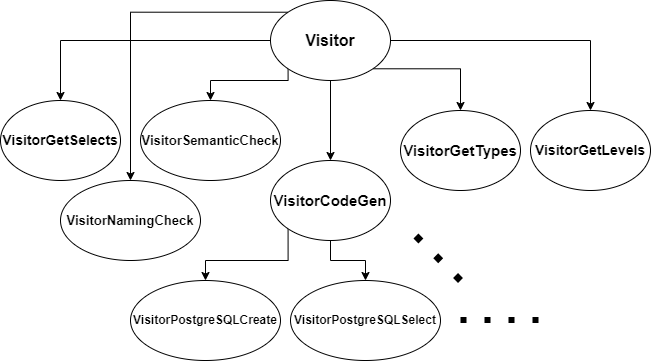
\includegraphics[width=0.7\textwidth]{Graphics/visitorfixed.drawio.png}
    \caption{Jerarqu\'ia de Visitors}
    \label{fig:visitors}
\end{figure}

La clase \textbf{Visitor} es la ra\'iz de la jerarqu\'ia. Es una clase abstracta en la que se definen los m\'etodos 
\textbf{visit} que deben tener todas las clases herederas. En particular, hay un \textbf{visit} por cada tipo de 
nodo del AST. 

\begin{lstlisting}[label={code:visitors}, caption={Clase Visitor}, language={python}]
    class Visitor(metaclass = abc.ABCMeta):
        @abc.abstractmethod
        def visit_dimensional_model(self, dimensional_model): pass 

        @abc.abstractmethod
        def visit_attribute(self, attribute): pass

        @abc.abstractmethod
        def visit_attr_function(self, attr_func): pass

        @abc.abstractmethod
        def visit_agg_attr(self, agg_attr): pass

        @abc.abstractmethod
        def visit_attr_expression(self, attr_expression): pass

        @abc.abstractmethod
        def visit_dimensional_table(self, dimensional_table): pass
\end{lstlisting}

Las instancias de las clases \textbf{VisitorSemanticCheck}, \textbf{VisitorNamingCheck}, \textbf{VisitorGetTypes} 
son las encargadas de realizar
controles sem\'anticos sobre el c\'odigo del script del DSL analizado. Las instancias de \textbf{VisitorSemanticCheck} realiza los siguientes 
chequeos:

\begin{itemize}
    \item Revisa si en el esquema estrella definido existe al menos una dimensi\'on y una tabla de hechos.
    \item Se asegura que las tablas definidas tengan al menos un atributo v\'alido.
    \item Se asegura que todas las tablas tengan definidas al menos una llave primaria.
\end{itemize}

Las instancias de \textbf{VisitorNamingCheck} se encargan de recorrer el AST y verificar que: 

\begin{itemize}
    \item En las dimensiones o tablas de hecho no existan dos atributos definidos con el mismo nombre.
    \item Los atributos compuestos definidos tengan asignados un alias para su correcta identificaci\'on.
\end{itemize}

Las instancias de \textbf{VisitorGetTypes} son las responsables de verificar el buen uso de los tipos en el 
c\'odigo del DSL adem\'as de recolectar el tipo de cada atributo declarado en cada dimensi\'on y 
tabla de hechos, 
informaci\'on necesaria para el proceso de generaci\'on de c\'odigo. En particular realizan 
las siguientes verificaciones: 

\begin{itemize}
    \item Verifica que los atributos compuestos definidos se les haya especificado su tipo.
    \item En el caso de las llaves for\'aneas comprueba que tanto las tabla referenciada como el atributo 
        referenciado est\'en previamente declarados en el esquema estrella y que adem\'as la llave for\'anea 
        y el atributo referenciado coincidan en tipo.
\end{itemize}

Las instancias de \textbf{VisitorGetSelects} se encargan de recorrer el AST y por cada dimensi\'on o tabla 
de hechos recolectan las tablas y los atributos que hay que seleccionar de la fuente de datos 
para poblar dicha dimensi\'on o tabla de hechos. A partir de esta informaci\'on se confeccionan las consultas 
que se realizan a los \'arboles de join para obtener el join necesario para el proceso de poblaci\'on.

Las instancias de \textbf{VisitorGetLevel} son las encargadas de recopilar los niveles de cada uno de los 
atributos de las tablas del esquema estrella. Esta informaci\'on luego se exportar\'a al almac\'en de datos 
destino en forma de una tabla de metadatos llamada \textbf{level\_metadata}. Dicha tabla tendr\'a tres atributos: 
\textbf{table\_name}, \textbf{attribute\_name} y \textbf{level}. El primero es el nombre de la tabla del esquema 
estrella, el segundo es el nombre del atributo y el tercero es un entero que representa el nivel del atributo 
en la jerarqu\'ia de la tabla con nombre \textbf{table\_name}.

La clase \textbf{VisitorCodeGen} es una clase abstracta de la que heredar\'an todos los visitors que 
se encarguen de generar c\'odigo. Hereda de la clase \textbf{Visitor} y la extiende pues incorpora un 
m\'etodo para exportar las consultas generadas.

\begin{lstlisting}[label={code:vcodegen}, caption={Clase VisitorCodeGen}, language={python}]
    class VisitorCodeGen(Visitor):
        def visit_dimensional_model(self, dimensional_model):
            return super().visit_dimensional_model(dimensional_model)
        def visit_dimensional_table(self, dimensional_table):
            return super().visit_dimensional_table(dimensional_table)
        def visit_attr_expression(self, attr_expression):
            return super().visit_attr_expression(attr_expression)
        def visit_attribute(self, attribute):
            return super().visit_attribute(attribute)
        def visit_attr_function(self, attr_func):
            return super().visit_attr_function(attr_func)
        def visit_agg_attr(self, agg_attr):
            return super().visit_agg_attr(agg_attr)

        @abc.abstractmethod
        def export_querys(self): pass
\end{lstlisting}

La generaci\'on de c\'odigo es otro de los puntos de dependencia del prototipo con los sistemas de gesti\'on 
de bases de datos. Específicamente, las consultas de selecci\'on dependen del sistema de gestión de bases 
de datos de la fuente, pues estas se encargan de extraer los datos para la poblaci\'on, y las consultas 
de creaci\'on dependen del sistema de gestión de bases de datos del almac\'en de datos de destino, pues 
son las responsables de crear las tablas del esquema estrella en sistema destino. Para resolver esta dependencia 
se implementa un visitor para la generaci\'on de las consultas de selecci\'on y un visitor para la generaci\'on 
de las consultas de creaci\'on, por cada sistema de gesti\'on de bases de datos, como se muestra en la 
figura \ref{fig:visitors}. De esta forma, cada tipo de consulta la genera el visitor que le corresponde 
al sistema de gestion de bases de datos de la fuente o del destino. En esta primera versi\'on del prototipo 
se implementaron los visitors de generaci\'on de c\'odigo para PostgreSQL.

Las instancias de la clase \textbf{VisitorPostgreSQLCreate} son las encargadas de generar las 
consultas de creaci\'on de las tablas del esquema estrella para el sistema gestor PostgreSQL. En la 
declaraci\'on de los atributos 
dentro de la consulta se utiliza la informaci\'on recolectada por \textbf{VisitorGetTypes} para 
especificar los tipos de los atributos que se van a crear. Pero las instancias de \textbf{VisitorGetTypes} 
recolectan los tipos que maneja el DSL, por tanto cada instancia de \textbf{VisitorPostgreSQLCreate} 
tiene un diccionario que mapea los tipos del DSL a los tipos de PostgreSQL.

Las instancias de la clase \textbf{VisitorPostgreSQLSelect} generan las consultas de selecci\'on para 
el sistema gestor PostgreSQL. Reciben los joins seleccionados por el usuario para cada tabla del esquema 
estrella conforman las consultas de selecci\'on.

\subsection{Interfaz de Usuario}

Para la implementaci\'on de la interfaz de usuario se utiliz\'o la biblioteca Streamlit de python. Esta biblioteca 
permite la implementaci\'on de aplicaciones web mediante la definici\'on de scripts de python en donde se 
definan los componentes de las p\'aginas de la aplicaci\'on mediante la API de Streamlit. Adem\'as proporciona un 
servidor para alojar la aplicación e interactuar con ella. La interfaz de usuario de la aplicaci\'on cuenta 
con cuatro p\'aginas. En las secciones siguientes se explicar\'a el contenido y responsabilidad de cada p\'agina. 
La p\'agina principal se define en el directorio ra\'iz de la aplicaci\'on y el resto de las p\'aginas dentro 
de una carpeta llamada \textbf{pages}.

\subsubsection{Main Page}

Esta es la p\'agina principal de la aplicaci\'on. El script \textbf{Main\_Page.py} le da definici\'on 
a los componentes de la p\'agina. Aqu\'i el usuario deber\'a establecer conexi\'on con un servidor de 
base de datos fuente y escoger si desea realizar un proceso de recomputaci\'on de la conexi\'on. El 
proceso de recomputaci\'on conciste en crear una instancia de crawler para explorar la base de datos 
fuente, crear la base de datos de Neo4j correspondiente al esquema de la fuente de datos en el Cat\'alogo 
de Datos, exportar el grafo de join y los \'arboles de join derivados. Como se expuso en el cap\'itulo 
\ref{chapter:proposal} este c\'omputo es costoso, por tanto solo est\'a pensado para realizarse la primera 
vez que se descubre la base de datos fuente o cuando el esquema de la misma sufra cambios y por tanto 
el Cat\'alogo de Datos, el grafo de join y los \'arboles de join son inv\'alidos y nececitan ser recalculados. 
Adem\'as, la pagina cuenta con un formulario para registrar nuevos servidores de base de datos. La informaci\'on 
de los servidores el almacenada en la ruta \textbf{data/connections} en formato json.

\subsubsection{Metadata}

En esta p\'agina se muestran los metadatos recopilados por el Crawler y adem\'as im\'agenes del 
grafo de join y los \'arboles de join derivados. El script de esta p\'agina es \textbf{Metadata.py}.

\subsubsection{Query Generator}

En esta p\'agina se mostraran las consultas generadas. Primero se selecciona un script del DSL que 
define un esquema estrella a poblar. Luego se debe escoger por cada tabla del esquema estrella el 
join que mejor se ajuste para la extracci\'on de los valores. La selecci\'on se realiza a trav\'es 
de componentes en la interfaz de usuario. Una vez seleccionado los joins aparecer\'a un bot\'on 
para comenzar el proceso de generaci\'on de consultas y al tocarlo se mostraran las consultas 
de creaci\'on y de selecci\'on para cada tabla del esquema estrella, as\'i como la consulta 
para crear y poblar la tabla de metadatos \textbf{level\_metadata}. Las consultas generadas 
son almacenadas en la ruta \textbf{data/script} haciendo posible su recuperaci\'on y descarga por parte del usuario. 
Todo el proceso de generaci\'on y an\'alisis del script del DSL es mediado por la clase \textbf{Orchestrator} 
presente en \textbf{orchestrator.py}. 

\begin{lstlisting}[label={code:orchestrator}, caption={Clase Orchestrator}, language={python}]
    class Orchestrator:
        def __init__(self, dbname, dwname, source_sgbd, target_sgbd, script) -> None:
            # Omitted Implementation

        def parse_code(self, code):
            # Omitted Implementation

        def compute_joins(self):
            # Omitted Implementation

        def generate_querys(self, selected_joins):
            # Omitted Implementation
\end{lstlisting}

Los campos de la clase son \textbf{dbname} que es el nombre de la base de datos fuente, 
\textbf{dwname} que es el nombre del almac\'en de datos de destino, \textbf{source\_sgbd} y 
\textbf{target\_sgbd} son los sistemas gestores de bases de datos de la fuente de datos y 
del almac\'en de datos de destino, y \textbf{script} es una cadena de texto con el c\'odigo 
de definici\'on del esquema estrella a poblar.

El m\'etodo \textbf{parse\_code} se encarga de tomar el c\'odigo en \textbf{script}, parsearlo 
con la instancia de parser de \textbf{PLY} y as\'i obtener el AST del c\'odigo de \textbf{script}. 
Luego dicho AST se somete a los recorridos de todos los visitors explicados anteriormente. Si dichos 
recorridos encuentran anomal\'ias en el c\'odigo estas son escritas en el archivo \textbf{dsl\_log.log} 
para luego mostrarlas al usuario. Si no se detectan anomal\'ias entonces se pasa a computar los joins. 

El m\'etodo \textbf{compute\_joins} recupera los \'arboles de joins almacenados para la base de datos 
feunte en cuesti\'on. Luego con la informaci\'on recopilada por la instancia de visitor \textbf{VisitorGetSelect}, 
por cada tabla del esquema estrella se computan un conjunto de posibles joins para conformar la consulta 
de selecci\'on, utilizando el algoritmo propuesto en el capitulo \ref{chapter:proposal} para la fase 
de consulta a los \'arboles de join. Luego de este proceso, el usuario mediante la interfaz debe seleccionar 
los joins de su conveniencia para la conformaci\'on de las consultas de selecci\'on. 

El m\'etodo \textbf{generate\_querys} se encarga de tomar los joins seleccionados por el usuario para 
cada tabla del esquema estrella y conformar las consultas de creaci\'on y de selecci\'on. El visitor 
correspondiente para la generaci\'on de ambas consultas se selecciona utilizando los campos 
\textbf{source\_sgbd} y \textbf{target\_sgbd}. Las consultas generadas son mostradas en la interfaz y es 
posible su descarga para que el usuario disponga de ellas para construir manualmente un pipeline v\'alido. 
Las consultas son descargadas en archivos separados con extensi\'on .sql.

\subsubsection{Logs}

Finalmente, en esta p\'agina se muestran los errores en la escritura del script de definici\'on del esquema
estrella encontrados por los visitors.